 \documentclass{article}
\usepackage{fancyhdr} % Required for custom headers
\usepackage{lastpage} % Required to determine the last page for the footer
\usepackage{extramarks} % Required for headers and footers
\usepackage{graphicx} % Required to insert images
\usepackage{lipsum} % Used for inserting dummy 'Lorem ipsum' text into the template
\usepackage{amsmath,amsthm,amsxtra}
\usepackage{physymb}
\usepackage{calligra}
% Margins
\topmargin=-0.45in
\evensidemargin=0in
\oddsidemargin=0in
\textwidth=6.5in
\textheight=9.0in
\headsep=0.25in 
\setlength{\parindent}{10ex}
\linespread{1.1} % Line spacing

% Set up the header and footer
\pagestyle{fancy}
\lhead{\hmwkAuthorName} % Top left header
\chead{\courseTitle\ : \hmwkTitle} % Top center header
\rhead{\firstxmark} % Top right header
\lfoot{\lastxmark} % Bottom left footer
\cfoot{} % Bottom center footer
\rfoot{Page\ \thepage\ of\ \pageref{LastPage}} % Bottom right footer
\renewcommand\headrulewidth{0.4pt} % Size of the header rule
\renewcommand\footrulewidth{0.4pt} % Size of the footer rule

%\setlength\parindent{0pt} % Removes all indentation from paragraphs

%----------------------------------------------------------------------------------------
%	DOCUMENT STRUCTURE COMMANDS
%	Skip this unless you know what you're doing
%----------------------------------------------------------------------------------------

% Header and footer for when a page split occurs within a problem environment
\newcommand{\enterProblemHeader}[1]{
\nobreak\extramarks{#1}{#1 continued on next page\ldots}\nobreak
\nobreak\extramarks{#1 (continued)}{#1 continued on next page\ldots}\nobreak
}

% Header and footer for when a page split occurs between problem environments
\newcommand{\exitProblemHeader}[1]{
\nobreak\extramarks{#1 (continued)}{#1 continued on next page\ldots}\nobreak
\nobreak\extramarks{#1}{}\nobreak
}

\setcounter{secnumdepth}{0} % Removes default section numbers
\newcounter{homeworkProblemCounter} % Creates a counter to keep track of the number of problems
\newcommand{\homeworkProblemName}{}
\newenvironment{homeworkProblem}[1][Problem \arabic{homeworkProblemCounter}]{ % Makes a new environment called homeworkProblem which takes 1 argument (custom name) but the default is "Problem #"
\stepcounter{homeworkProblemCounter} % Increase counter for number of problems
\renewcommand{\homeworkProblemName}{#1} % Assign \homeworkProblemName the name of the problem
\section{\homeworkProblemName} % Make a section in the document with the custom problem count
\enterProblemHeader{\homeworkProblemName} % Header and footer within the environment
}{
\exitProblemHeader{\homeworkProblemName} % Header and footer after the environment
}

\newcommand{\problemAnswer}[1]{ % Defines the problem answer command with the content as the only argument
\noindent\framebox[\columnwidth][c]{\begin{minipage}{0.98\columnwidth}\begin{center}#1\end{center}\end{minipage}} % Makes the box around the problem answer and puts the content inside
}

\newcommand{\homeworkSectionName}{}
\newenvironment{homeworkSection}[1]{ % New environment for sections within homework problems, takes 1 argument - the name of the section
\renewcommand{\homeworkSectionName}{#1} % Assign \homeworkSectionName to the name of the section from the environment argument
\subsection{\homeworkSectionName} % Make a subsection with the custom name of the subsection
\enterProblemHeader{\homeworkProblemName} % Header and footer within the environment
}{
\enterProblemHeader{\homeworkProblemName} % Header and footer after the environment
}

%----------------------------------------------------------------------------------------
%	NAME \longmapstoAND CLASS SECTION
%----------------------------------------------------------------------------------------

\newcommand{\hmwkTitle}{Quiz \#2, Problem 2} % Assignment title
\newcommand{\hmwkDueDate}{} % Due date
\newcommand{\courseTitle}{ECE 106 - Tutorial} % Course/class
\newcommand{\hmwkClassInstructor}{Taught by: Dr. Firas Mansour and Dr. Bajcsy} % Teacher/lecturer
\newcommand{\hmwkAuthorName}{John Rinehart} % Your name
\newcommand{\sudentNumber}{} % Your name
\newcommand{\position}{PhD student in Physics Department}

%----------------------------------------------------------------------------------------
%%-----------------------------------------------------------------------------------------

%%%%%%%%%%
\newcommand{\red}[1]{\textcolor[rgb]{1,0,0}{#1}}
\newcommand{\blu}[1]{\textcolor[rgb]{0,0,1}{#1}}
\newcommand{\bs}[1]{\boldsymbol{#1}}
%\newcommand{\V}[1]{\bm{#1}}
\newcommand{\V}[1]{\Vec{#1}}
\newcommand{\A}[1]{\Hat{#1}}
\newcommand{\W}[1]{\widehat{#1}}
\newcommand{\T}[1]{\widetilde{#1}}

%\newcommand{\pd}[2]{\dfrac{\partial #1}{\partial #2}}
\newcommand {\ppds}[2]{\dfrac{\partial^2 {#1}}{\partial {#2}^2}}
\newcommand{\ppdss}[2]{\dfrac{\partial^2}{\partial #1 \partial #2}}
\newcommand{\pdtt}[3]{\dfrac{\partial^2 {#1}}{\partial {#2} \partial {#3}}}

\newcommand{\fpd}[2]{\frac{\partial #1}{\partial #2}}
\newcommand{\fpds}[1]{\frac{\partial}{\partial #1}}

\newcommand{\ignore}[1]{}

\newcommand{\der}[2]{\frac{d{#1}}{d{#2}}}
\newcommand{\vt}[1]{\Vec{\mathcal{#1}}}
\newcommand{\VP}[1]{\Vec{\mathbf{#1}}}
\newcommand{\vp}[1]{\mathbf{#1}}
\newcommand{\phas}[1]{\angle{#1}^{\circ}}
\newcommand{\er}{\epsilon_{r}}
\newcommand{\mr}{\mu_{r}}
\newcommand{\Lrw}{\Longrightarrow}
\newcommand{\refeq}[1]{(\ref{#1})}
%\newcommand{\abs}[1]{\left| #1\right|}
\newcommand{\ket}[1]{|#1\rangle}
\newcommand{\bra}[1]{\langle #1| }
\newcommand{\intas}{\int\limits_{all\;space}}
\newcommand{\intsradial}[3]{\int\limits_{#1}^{#2} #3 r^2 \mathrm{d} r}
\newcommand{\intspolar}[3]{\int\limits_{#1}^{#2} #3 sin(\theta) \mathrm{d} \theta}
\newcommand{\intsazim}[3]{\int\limits_{#1}^{#2} #3 \mathrm{d} \phi}
\newcommand{\intcz}[3]{\int\limits_{#1}^{#2} #3 \mathrm{d} z}
\newcommand{\intcx}[3]{\int\limits_{#1}^{#2} #3 \mathrm{d} x}
\newcommand{\intcy}[3]{\int\limits_{#1}^{#2} #3 \mathrm{d} y}
\newcommand{\intavcart}[1]{\int \limits_{all\; space} #1 \, \mathrm{d} x \mathrm{d} y \mathrm{d} z}
\newcommand{\bracket}[2]{\langle#1|#2\rangle }
\newcommand*{\myalign}[2]{\multicolumn{1}{#1}{#2}}

\newcommand*\diff{\mathop{}\!\mathrm{d}}
\newcommand*\Diff[1]{\mathop{}\!\mathrm{d^#1}}

% New definition of square root:
% it renames \sqrt as \oldsqrt
\let\oldsqrt\sqrt
% it defines the new \sqrt in terms of the old one
\def\sqrt{\mathpalette\DHLhksqrt}
\def\DHLhksqrt#1#2{%
\setbox0=\hbox{$#1\oldsqrt{#2\,}$}\dimen0=\ht0
\advance\dimen0-0.2\ht0
\setbox2=\hbox{\vrule height\ht0 depth -\dimen0}%
{\box0\lower0.4pt\box2}}

%%%---
\newcommand\ointint{\begingroup
\displaystyle \unitlength 1pt
\int\mkern-7.2mu
\begin{picture}(0,3)
\put(0,3){\oval(10,8)}
\end{picture}
\mkern-7mu\int\endgroup}
%%%----
\providecommand{\abs}[1]{\lvert#1\rvert}
\providecommand{\norm}[1]{\lVert#1\rVert}

%%%%%%%%%%%%%%%

%---Packeges------------------------------------------------------------------
 %------------------------------------------------------
\usepackage{pdfsync}
\usepackage[T1]{fontenc}
\usepackage{lmodern}
\usepackage[english]{babel}
\usepackage[utf8,latin1]{inputenc}
\usepackage[T1]{fontenc}
\usepackage[usenames,dvipsnames]{pstricks}
\usepackage{epsfig}
\usepackage{pst-grad} % For gradients \usepackage{pst-plot} % For axes
\usepackage{pifont}
\usepackage{amsfonts}
\graphicspath{{IMG/}}
 \usepackage[absolute,overlay]{textpos}
 \usepackage{graphicx}
 \usepackage[bookmarks=false,pdffitwindow]{hyperref}
 \usepackage{tikz}
 \usepackage{xcolor}
 \usepackage{calc}
\usepackage{chngcntr}
\usepackage{microtype}

% Matlab code section obtained from StackExchange: http://tex.stackexchange.com/questions/75116/what-can-i-use-to-typeset-matlab-code-in-my-document
\usepackage{listings}
\usepackage{color} %red, green, blue, yellow, cyan, magenta, black, white
\definecolor{mygreen}{RGB}{28,172,0} % color values Red, Green, Blue
\definecolor{mylilas}{RGB}{170,55,241}

\lstset{language=Matlab,%
    %basicstyle=\color{red},
    breaklines=true,%
    morekeywords={matlab2tikz},
    keywordstyle=\color{blue},%
    morekeywords=[2]{1}, keywordstyle=[2]{\color{black}},
    identifierstyle=\color{black},%
    stringstyle=\color{mylilas},
    commentstyle=\color{mygreen},%
    showstringspaces=false,%without this there will be a symbol in the places where there is a space
    numbers=left,%
    numberstyle={\tiny \color{black}},% size of the numbers
    numbersep=9pt, % this defines how far the numbers are from the text
    emph=[1]{for,end,break},emphstyle=[1]\color{red}, %some words to emphasise
    %emph=[2]{word1,word2}, emphstyle=[2]{style},    
}

%----------------------------------------------------------------
\numberwithin{equation}{section}
\renewcommand{\theequation}{\arabic{equation}}



%%------------------------------------------------------------------------------------------
%	TITLE PAGE
%----------------------------------------------------------------------------------------

\title{
\vspace{2in}
\textmd{\textbf{\courseTitle\\ \vspace{0.5in}\hmwkTitle}}\\
\vspace{0.5in}\large{{\hmwkClassInstructor}}
\vspace{3in}
}
\author{\textbf{\hmwkAuthorName}\\ 
}

%\date{\currenttime} % Insert date here if you want it to appear below your name

%----------------------------------------------------------------------------------------
\begin{document}

\maketitle


\newpage
\tableofcontents
\newpage

%----Problems-------
\begin{homeworkProblem}[Quiz 2, Problem 2] 
    Okay, the problem of solving for the z-component of the electric
    field generated by a charged disk seemed to be difficult for you
    guys. Let me discuss a few ways in which this problem could be
    solved.
    
    The first approach that I will use will be to establish the
    electric field set up by a ring centered around the z-axis. Then, I
    will integrate over an infinite number of rings whose radius varies
    smoothly from 0 to the radius of the disk.

    The second approach that I will use will be to establish the
    electric field from a disk directly using polar coordinates. I will
    integrate around the disk (in the angular direction) and I will
    integrate radially outward (from 0 to R, the radius of the disk).
    This involves the use of the differential area alement $\diff a$ in
    polar coordinates. I will try my best to explain the origins of this
    differential area element. That may go in an appendix at the end.

    \begin{homeworkSection}{Approach 1}
        Okay, so I'm going to first start by solving for the electric
        field established by a uniformly charged ring. The ring will
        have a constant charge per unit length, $\lambda$, such that the
        total charge on the ring is $2\pi R \lambda = Q$. My approach
        will be to chop up the ring into a bunch of infinitesimal point
        charges $\diff q'$ and evaluate the electric field, $\diff \vec{E}$,
        generated by each of these infinitesimal point charges. Once I
        have this contribution to the electric field I will integrate
        over all the infinitesimal point charges to find the net
        electric field $\vec{E} = \int \diff \vec{E}$. 

        \begin{figure}[t]
            \centering    
            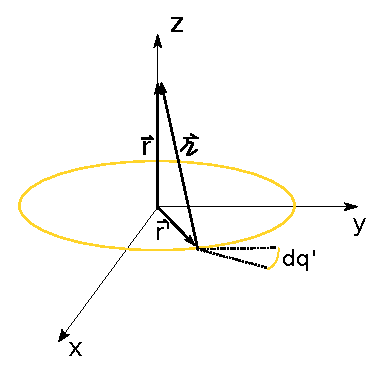
\includegraphics{./img/ringofcharge.eps}
            \caption{Ring of charge centered along z-axis}
            \label{fig:roc.eps}
        \end{figure}

        The key to starting to write this integral is to realize that
        each infinitesimal check of charge $\diff q'$ is like a little point
        charge located at position $r'$ (see figure \ref{fig:roc.eps})
        and, as such, the electric field contribution due a particular
        chunk of charge, $\diff q'$, looks like:

        \[ \diff \vec{E}(\vec{r}) = \frac{k \diff q'}{|\vec{\scriptr}|^2}
        \hat{\scriptr} \]

        Now, $\diff q'$ really describes the position of a chunk of charge
        $\diff q'$ located at $\vec{r'}$. The infinitesimal chunk of charge
        can be written as $\diff q' = \lambda \diff l'$, where $\diff
        l'$ is an infinitesimal arc length along the path of the ring.

        Thus, my expression for $\diff \vec{E}(\vec{r})$ looks like
        
        \[ \diff \vec{E}(\vec{r}) = \frac{k \lambda \diff l'}{|\vec{\scriptr}|^2}
        \hat{\scriptr} \]

        But, $\diff l'$ just represents a little arc length. We know
        that an arc length $s$ can be related to the radius of the
        circle and the swept (subtended) angle, $\theta$ can be written
        as $s = R \theta$. Thus, I will write the arc length $\diff l'$
        as $\diff l' = R \diff \theta'$ so that $\diff \vec{E}(\vec{r})$
        becomes:


        \[ \diff \vec{E}(\vec{r}) = \frac{k \lambda R \diff
        \theta'}{|\vec{\scriptr}|^2} \hat{\scriptr} \]

        Now, our expression is looking more and more like something we
        can integrate. However, we should really right $\vec{\scriptr}$
        in terms of something we know. What is $\vec{\scriptr}$?
        Remember, this vector points from the point where the charge
        that we're considering is located to the point where we would
        like to evaluate the electric field. Thus, in terms of
        $\vec{r}$, the vector that points from the origin to where we
        would like to evaluate the electric field and $\vec{r'}$, the
        vector that points from the origin to the chunk of charge we're
        considering $\vec{\scriptr} = \vec{r}-\vec{r'}$. In order to put
        this into my expression for $\diff \vec{E}$ I need to scale
        thetope and bottom by the magnitude of $\vec{\scriptr}$ to get
        rid of that pesky unit vector. Doing this yields:
        
        \[ \diff \vec{E}(\vec{r}) = \frac{k \lambda R \diff
        \theta'}{|\vec{\scriptr}|^3} \vec{\scriptr} \]

        Performing my substitution for $\vec{\scriptr}$ yields:

        \[ \diff \vec{E}(\vec{r}) = \frac{k \lambda R \diff
        \theta'}{|\vec{r}-\vec{r'}|^3} (\vec{r} - \vec{r'}) \]

        Now, can we simplify this expression at all before we integrate?
        Yes! We know that $\vec{r} = z \hat{z}$ since we are only
        solving for the electric field along the z-axis. We also know
        that $|\vec{\scriptr}|$ is $\sqrt{R^2+z^2}$ (look at
        \ref{fig:roc.eps})
        Performing these substitutions yields:

        \[ \diff \vec{E}(z) = \frac{k \lambda R \diff
        \theta'}{(R^2+z^2)^{1.5}} (z \hat{z}- \vec{r'}) \]

        Now, we can almost perform this integral. We just need an
        expression for $\vec{r'}$ in terms of $\theta'$ so that we can
        perform the integral over $\theta'$. But, $\vec{r'} =
        R\cos(\theta')\hat{x} - R\cos(\theta')\hat{y}$. This can be seen
        by considering how $\vec{r'}$ must change direction as a
        function of $\theta'$. Now, we just plug this into our previous
        expression and integrate over $\theta'$ from $0 \rightarrow
        \pi/2$.

        \[ \vec{E}(z) = \int\limits_0^{2\pi} k \lambda R \frac{ \diff
        \theta'}{(R^2+z^2)^{1.5}} (z \hat{z}-
        R\cos(\theta')\hat{x}+R\cos(\theta')\hat{y}) \]

        Now, k and $\lambda$ are constants that I can pull out of the
        integral. The integrals over $\cos\theta'$ and $\sin\theta'$ I
        already know are going to go away. I know this because
        $\int_0^{2\pi} \cos\theta \diff \theta = \int_0^{2\pi}
        \sin\theta \diff \theta = 0 $. Thus, only the $\hat{z}$
        component survives the integral (like we'd expect) and the
        integral reduces to:

        \[ \vec{E}(z) = \int\limits_0^{2\pi} k \lambda R \frac{ \diff
        \theta'}{(R^2+z^2)^{1.5}} z \hat{z} \]

        Notice that everything inside the integral is a constant with
        respect to $\theta'$ except for our integration differential
        $\diff \theta'$. Thus, the integral is just:

        \[ \vec{E}(z) = \frac{k\lambda R 2\pi z
        \hat{z}}{(R^2+z^2)^{1.5}} \]

        This looks a little ugly. Once we realize that $2\pi R \lambda$
        is just $Q$, thet total charge on the ring (the charge per unit
        length on the ring times the total length of the ring) we can
        simplify this to:

        \[ \vec{E}(z) = \frac{k Q }{(R^2+z^2)^{1.5}} z\hat{z} \]

        Note that this expression depends on the radius of the ring. Our
        next goal will be to integrate over a bunch of rings with
        different radii to obtain the electric field along the z-axis
        due to a charged disc. Thus, I'm going to chop the electric
        field for the disc up into a bunch of rings.
   
        \[ \diff \vec{E}(z) = \frac{k dQ}{(R^2+z^2)^{1.5}} z\hat{z} \]

        \begin{figure}[t]
            \begin{center}
                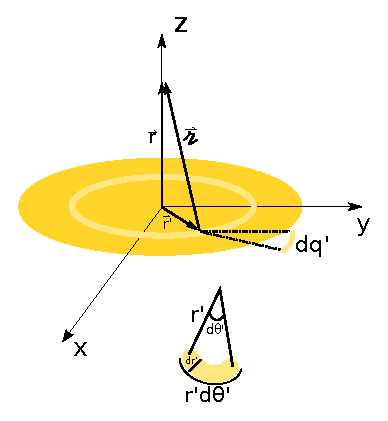
\includegraphics{./img/discofcharge.eps}
            \end{center}
            \caption{Disc of charge broken up into rings}
            \label{fig:doc.eps}
        \end{figure}

        What is dQ? Well, dQ is me treating each ring as a chunk of
        charge that generates a little portion of the total electric
        field. Now, since I'm integrating over rings to form a disc I
        need to give these rings some infinitesimal width. The disc will
        be formed of a bunch of rings of infinitesimal width. A ring of
        infinitesimal width and of radius $R'$ will have an amount of
        charge equal to $2 \pi R' dR' \sigma$ (see \ref{fig:doc.eps} and
        allow $\diff \theta'$ to be $2 \pi$ - you might argue that this
        is not an infinitesimal quantity\dots well it turns out that
        this doesn't matter. It's still the area of that ring: $2\pi r'
        dr'$). What is $\sigma$? It's the surface charge density. Since
        we're considering areas of charge, now, we need to consider area
        charge densities. Think about whether a relationship can be
        drawn between $\lambda$ and $\sigma$. Let's try to write down
        the integral now that we know what $\diff Q$ is.

        \[ \vec{E}(z) = \int_0^{R_{disc}} \diff \vec{E}(z) =
        \int_0^{R_{disc}}\frac{k 2 \pi R' dR' \sigma}{(R'^2+z^2)^{1.5}}
        z\hat{z} \]

        Now, this integral is not hard to solve. I'll pull out the
        constants so that the math is a little more transparent. 
        
        \[ \vec{E}(z) = \int_0^{R_{disc}} \diff \vec{E}(z) =
        2\pi \sigma z \hat{z} \int_0^{R_{disc}}\frac{R' dR'
        }{(R'^2+z^2)^{1.5}} \tag{1} \]
        
        Now, I solved this using WolframAlpha but this type of integral
        can be solved with a simple u-substitution (allow $u = R'^2 +
        z^2$ so that $\frac{\diff u}{\diff r} = 2 R' dR'$).

        The final result, after doing all of this is that:

        \[ \vec{E}(z) = k\sigma 2\pi \bigg( 1 - \frac{z}{z^2+R_{disc}^2}
        \bigg)\hat{z} \]

        %\[ \vec{E}_{disc}(z) = \int_0^{R_{disc}}\frac{k Q(R) \diff R
        %}{(R^2+z^2)^{1.5}} z\hat{z} \]

        %The reason that Q is now a function of R is that we want to
        %describe the electric field generated by a bunch of rings. In
        %order that the disc have a uniform charge density over its area,
        %each of the constituent rings need a uniform charge density over
        %their own circumferences. Thus, for a larger ring, there exists
        %more charge on that ring.

        %What is $Q(R)$? Well that's a good question. We know that $Q =
        %2\pi\lambda R$. This must be $Q(R)$. That makes sense. Let's
        %plug this in.
        
        \end{homeworkSection}
    
    \begin{homeworkSection}{Approach 2}

        Now, that was super tedious. Let's try this another way. Let's
        now break the disc up into a little bunch of patches of area
        $da$ instead of a bunch of rings of infinitesimal thickness. If
        we do this, we need to think about how best to think about the
        area of the disc.
        
        If we break the disc up into a bunch of
        rectangular areas, $da$, like is done with Cartesian coordinates
        we will have a difficult time integrating over our disc (see
        %\ref{fig:patches.eps}
        . Our bounds will have to be over the area of the disc which
        require that we express the limits of our integral in terms of
        the equation of the circle. I don't really want to deal with $y
        = \pm \sqrt{1-x^2}$ in my limits.


        Instead, let's consider the patches of area to be little arcs of
        some finite thickness. See \ref{fig:doc.eps} for a decent visual
        explanation.  Now, it's easy to break up the area of our circle
        into little chunks. We will talk about a little chunk of area
        $da = (R \diff \theta)(\diff R)$. That is, the little chunk will
        have an arclength that is $R \diff \theta$ long and $\diff R$
        wide. That determines the area of this patch. You can convince
        yourself, easily, that this is a great way to think about areas
        when it comes to dealing with problems with circles in them.
        Let's integrate the area of a circle with these coordinates:

        \begin{align}
            A &= \int_0^R da \nonumber \\
            &=  \int_0^R \int_0^{2\pi} r \diff r \diff \theta
            \nonumber \\
            &= \int_0^R r \diff r \int_0^{2\pi} \diff \theta \nonumber \\
            &= \frac{r^2}{2}\big|_0^R \quad \theta\big|_0^{2\pi}
            \nonumber \\
            &= \pi R^2 \nonumber 
        \end{align}

        So, although this isn't a proof, it should at least be
        convincing evidence that maybe this is a good expression to use
        for the differential area element when we're dealing with
        circles. Now, I'm going to immediately write the integral we're
        going to solve since the approach is very similar to what we'va
        already done.

        \[ \vec{E}(z) = \int_0^{2\pi} \int_0^R \frac{k dq' (z \hat{z}-
        r'\cos(\theta')\hat{x}+r'\cos(\theta')\hat{y})}{(z^2+r'^2)^{1.5}}
        \]

        Now, $r'$ describes the distance the infinitesimal chunk of
        charge is away from the origin. $\theta$ describes the location
        of that chunk with respect to the x-axis. Thus, by sweeping over
        all $\theta': 0 \rightarrow 2\pi$ and all $r': 0 \rightarrow R$ we
        sweep over all the charge. Now, we just have to right $dq'$ in
        terms of $r'$ and $\theta'$ and we're good. But, $dq' = \sigma
        \diff a' = \sigma r' dr' \diff \theta'$, from the earlier
        discusson. The integral now reads:

        \[ \vec{E}(z) = \int_0^{2\pi} \int_0^R \frac{k \sigma r' dr'
        \diff \theta' (z \hat{z}-
        r'\cos(\theta')\hat{x}+r'\cos(\theta')\hat{y})}{(z^2+r'^2)^{1.5}}
        \]

       Right away I'm going to realize that the integral over the
       $\hat{x}$ and the $\hat{y}$ components go away because I'm
       integrating $\sin\theta'$ and $\cos\theta'$ over one period (from
       0 to $2\pi$).

        \[ \vec{E}(z) = \int_0^{2\pi} \int_0^R \frac{k \sigma r' dr'
        \diff \theta' (z \hat{z} }{(z^2+r'^2)^{1.5}}
        \]

        Now, the only $\theta'$ in my integral is the $\diff \theta'$.
        So, I can evaluate the integral over $\diff \theta'$ very
        easily. 

        \[ \vec{E}(z) = 2\pi \int_0^R \frac{k \sigma r' dr'
        (z \hat{z} }{(z^2+r'^2)^{1.5}}
        \]

        I then realize that this is the same integral as the one I was
        doing earlier (see Equation 1). Thus, the result must be the
        same. This is an easier, less confusing way to get the electric
        field for a disc along the z-axis.

    \end{homeworkSection}    
\end{homeworkProblem}

\setcounter{equation}{0}
---------------------
%\begin{homeworkProblem}[Quiz 3, Pr. 2]
    \textbf{Charge Q is uniformly distributed over the volume of a
    hollow sphere of inner radius a and outer radius b, as shown. r is
    the distance from the center of the hollow part (the geometrical
    center of the structure).}

    \begin{homeworkSection}{2a}
        \textbf{Find the electric field inside the hollow part.}
        \\
        
        \begin{figure}[t]
            \centering
            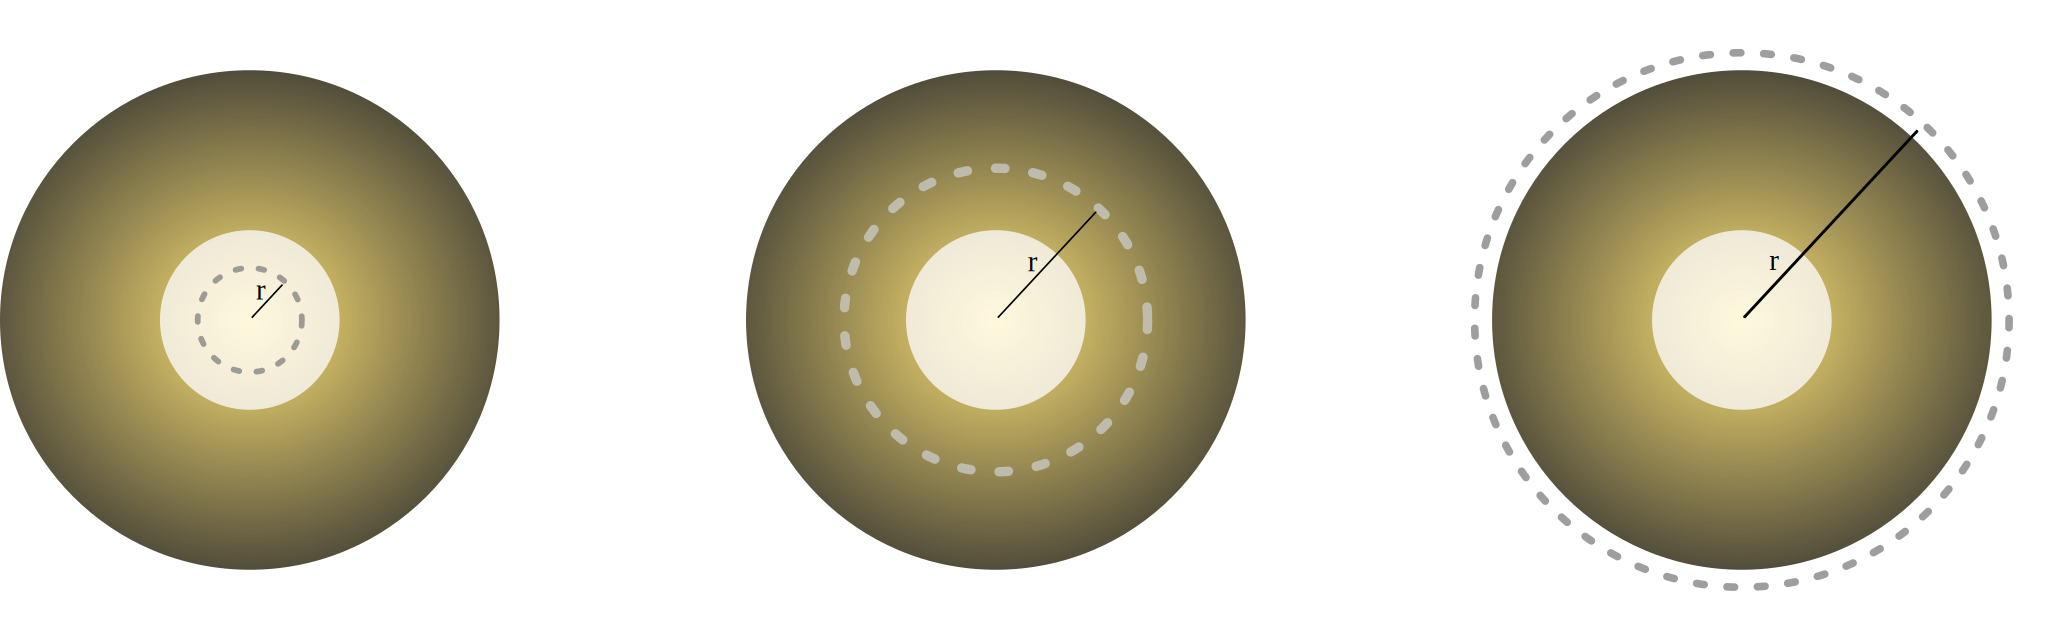
\includegraphics[width=.75\textwidth]{./img/gaussianspheres.pdf}
            \caption{Hollow, charged sphere with Gaussian spheres
            located within the hollow (left), within the charged region
            (right) and encompassing all of the charge in the sphere
            (right)}
            \label{fig:gaussianspheres.eps}
        \end{figure}

        This is a little more challenging than the previous, problems.
        Now, we are dealing with a continuous distribution of charge. In
        order to find the electric field we must use Gauss' law:
        $\oint\limits_{\text{surface}}
        \vec{E}\cdot\vec{da} = \frac{Q}{\epsilon_0}$. The way in which
        we'll use Gauss' law is we'll define a surface that takes
        advantage of the symmetry of the problem. We'll pick a surface
        whose differential area vector ($\vec{da}$) is in the same
        direction as the electric field, $\vec{E}$, for all the places
        at which we need to compute this integral. The most natural
        surface to use is a sphere.
        
        The spherical charge distribution should, through symmetry
        considerations, generate an electric field that is radially
        distributed. You can justify this by imagining rotating the
        sphere. If the sphere is perfectly symmetrical then there must
        be no way that you can tell what is ``up'' ,what is ``left'',
        etc. Thus, the electric field must be symmetric with respect to
        rotations. The only distrbution of vectors that accomplishes
        this is a radial distribution.
        
        Now, our surface, our ``Gaussian surface'', will be a sphere
        with a specified radius. In this part of the problem, we are
        only asked to compute the electric field in the region where
        $r<a$. That is, in the region where there is no electric charge.
        The way in which we'll calculate the electric field is to define
        a sphere of a certain radius ($r<a$) and we'll find out how much
        charge is enclosed inside that sphere. By relating the enclosed
        charge to the surface area of our sphere we can calculate the
        electric field. Watch:

        \begin{align}
            \label{}
            \Phi = \oint\limits_{\text{sphere}} \vec{E}\cdot\vec{da} =
            \frac{Q_{enc}}{\epsilon_0} \nonumber \\
            \oint\limits_{\text{sphere}} \vec{E}\cdot\vec{da} =
            \frac{\oint\limits_{\text{charge enclosed}}\rho dV}{\epsilon_0}
        \end{align}

        Note, that my Gaussian surface, this sphere, might enclose a
        distribution of charge. So, it's necessary for me to add up all
        the charge that might be enclosed by my sphere. That's the
        reason I have rewritten the right-hand side.

        Okay, now we can simplify the expression on the left-hand side
        of the above expression. $\vec{E}$ is, by symmetry
        considerations, directed radially outward. That is $\vec{E} =
        E(r) \hat{r}$. Now, I can also argue that by symmetry the
        magnitude of the electric field should be the same at all
        distances $r$ away from the origin. Thus, $E(r)$ is a constant
        and can be pulled out of the integral. The differential area
        element $\vec{da}$, by virtue of me having chosen a sphere as my
        Gaussian surface is $da \hat{r}$. So, it is in the same
        direction as the electric field. Thus, $\vec{E}(r) \cdot
        \vec{da} = E(r) da$, where $E(r)$ is a constant. Applying all
        these simplying results yields:

        \[
        \oint\limits_{\text{sphere}} \vec{E}\cdot\vec{da} = E(r)
        \oint\limits_{\text{sphere}} da
        \]

        The last expression is just asking for the total surface area of
        the sphere (the sum of all of the differential areas is the
        total area). Thus:
        
        \[
        E(r) \oint\limits_{\text{sphere}} da = E(r) 4\pi r^2
        \]

        Where $r<a$ is the radius of our Gaussian surface. Now, how much
        charge is enclosed by our Gaussian surface for $r<a$? Nothing!
        There is no charge for $r<a$. Thus
        $\frac{\oint\limits_{\text{charge enclosed}}\rho dV}{\epsilon_0} = $.
        Since $r \ne 0$ equation 1 (along with our simplifying
        expressions) informs us that $E(r)=0$ everywhere inside the
        hollow region (for all $r<a$). Thus, the answer to 1a is $E(r<a)
        = 0$.

    \end{homeworkSection}
    \begin{homeworkSection}{2c}
        \textbf{Solve for the electric field for outside of the sphere
        where $r>b$.}
        \\

        Okay, this part of the quiz is easier than 2b, which is why I'm
        solving it first. I will start by using equation 1, which still
        applies.
        
        \[
            \oint\limits_{\text{sphere}} \vec{E}\cdot\vec{da} =
            \frac{\oint\limits_{\text{charge enclosed}}\rho dV}{\epsilon_0}
        \]

        Okay, by the same arguments as before, I can rewrite the left
        hand side as:

        \[
            E(r)\oint\limits_{\text{sphere}} da =
            \frac{\oint\limits_{\text{charge enclosed}}\rho dV}{\epsilon_0}
        \]

        Now, though, the charge enclosed is not zero. In fact, for $r>b$
        we have enclosed all of the charge on the sphere. Can we prove
        this? Yes. Let's first consider how we would find the amount of
        enclosed charge $Q_{enc} = \oint\limits_{\text{charge enclosed
        }}\rho dV$ Well, how much charge is this? It's
        $Q = \rho * V_{\text{charged hollow sphere}}$.        What is
        the volume of the charged hollow sphere? Well, it's the volume
        of a sphere of radius $b$ minus the volume of a sphere of radius
        $a$ : $V_{\text{charged hollow sphere}} = \frac{4\pi}{3}b^3 -
        \frac{4\pi}{3}a^3$. What is $\rho$? $\rho =
        \frac{Q}{V_{\text{charged hollow sphere}}}$. It is the amount of
        charge stored per volume of the charged hollow sphere.
    
        \[
        \rho = \frac{Q}{\frac{4\pi}{3}b^3 - \frac{4\pi}{3}a^3}
        \]

        Note that this is not the same thing as:
       
        \[ \rho = \frac{Q}{\frac{4\pi}{3}(b - a)^3} \]
        
        because $(a-b)^3 \ne (a^3-b^3)$, in general. The best way to
        think about the volume (to avoid algebraic mistakes) is to
        subtract the volumes of two spheres.

        So, finally, what is the total charge enclosed by our Gaussian
        surface? Well, it's our charge density, $\rho$, times the volume
        of charge enclosed. Since our Gaussian surface is larger than
        the charged sphere, though, then $V_{\text{charged hollow
        sphere}} = \frac{4\pi}{3}b^3 - \frac{4\pi}{3}a^3$, the volume of
        the entire charged hollow sphere. And, finally, $Q_{enc} =
        \rho*V_{\text{charged hollow sphere}} = Q$, the total charge on the
        sphere.

        Okay, we already said this. It makes sense. Once our Gaussian
        surface is bigger than the charged hollow sphere then our
        Gaussian surface must enclose all of the charge. But, this mode
        of thinking will help us, later, when we try to solve 2b. Okay,
        now, $\rho$ is a constant so we can pull it out of the
        right-hand side of our expression for Gauss' law. Then, we're
        just integrating over the volume of our Gaussian surface. For a
        Gaussian surface with radius $r>b$, the Gaussian surface's
        volume is just $\frac{4\pi}{3} r^3$. Thus, our expression for
        Gauss' law can be reduced to:

        \[
            E(r) 4\pi r^2 = \frac{Q}{\epsilon_0}
        \]

        Now, $E(r) = \frac{Q}{4\pi\epsilon_0 r^2} = \frac{kQ}{r^2}$.
        This is an important result. Outside of a spherically symmetric
        charge distribution, the electric field looks like exactly that of
        a point charge located at the origin. How big is that point
        charge? Well, it's as big as the amount of charge stored in that
        spherically symmetric charge distribution. Okay, this is the
        answer for 2c. Let's tackle 2b.
        
    \end{homeworkSection}
    \begin{homeworkSection}{2b}

        Okay, we'll start with Gauss' law. I'll immediately apply the
        symmetry results to simplify the expression.

        \[
            E(r)\oint\limits_{\text{sphere}} da =
            \frac{\oint\limits_{\text{charge enclosed}}\rho dV}{\epsilon_0}
        \]

        We have the expression for $\rho$ from before.
        \[ \rho = \frac{Q}{\frac{4\pi}{3}(b^3- a^3)} \]

        Now, $\rho$ is a constant (uniform charge distribution), so I
        can pull this out of the integral. The integral on the left-hand
        side over $da$ is just the area of our Gaussian surface $\oint
        da = A = 4\pi r^2$, as usual. The most difficult thing in this
        problem is the integral over $dV$ in the right-hand side. This
        is not the volume of our Gaussian surface! We are trying to
        calculate the amount of enclosed charge. Thus, this volume
        should be the volume of the enclosed charge. At a distance $r$
        from the center, the amount of charge I have enclosed is

        \[
        V_{\text{charge enclosed}} = \frac{4\pi}{3}r^3 -
        \frac{4\pi}{3}a^3
        \]

        It's exactly the volume of my Gaussian surface \textbf{minus the
        volume of my Gaussian surface in which there is no charge}. This
        is the center of the hollow sphere. Substituting this yields:

        \[
        E(r)4\pi r^2  = \frac{1}{\epsilon_0} \bigg(
        \frac{Q}{\frac{4\pi}{3}b^3 - \frac{4\pi}{3}a^3}\bigg) \bigg( \frac{4\pi}{3}
        r^3 -\frac{4\pi}{3}a^3 \bigg)
        \]

        After a little algebra this can be rewritten as:

        \[
        E(r) = \frac{Q}{4\pi \epsilon_0 r^2} \frac{r^3-a^3}{b^3-a^3}
        \]

        This is the answer for problem 2b.
    \end{homeworkSection}
    \begin{homeworkSection}{2d}
        \textbf{Solve for the electric field at the outer surface where
        $r=b$.}
        \\

        Now, this problem is very simple. We just have to plug in $r=b$
        into our expressions for $E(r)$ from either part b or or part c.
        How come we can use either expression? Well, the electric field
        outside the sphere, for all $r>b$, is given by the answer in 2c.
        The electric field inside the sphere, for $a<r<b$, is given in
        2b. So, taking the limit as $r\rightarrow b$ both expressions
        should yield the same thing, if a limit exists. And, this is a
        fairly simple situation, that could be constructed fairly
        easily, so we hope a limit exists. It's easiest to plug $r=b$
        into the answer we got in 2c, but we could just as well plug it
        into 2b. If we do this, we obtain:

        \[
        E(b) = \frac{kQ}{b^2}
        \]
    \end{homeworkSection}
\end{homeworkProblem}

%\setcounter{equation}{0}
%--------------------- 
%\input{Problem3}
%\setcounter{equation}{0}
%----------------------
%%% ... %%%
%$\input{Problem4}
%\setcounter{equation}{0}

%\input{Problem5}
%\setcounter{equation}{0}
%\newpage
%\input{Appendix}
%%%\newpage
%%%\input{Mybib}


%----------------------------------------
\end{document}
